% Data flow diagram
% Author: David Fokkema
\documentclass{article}
\usepackage[margin=0.5in]{geometry}
\usepackage{mathtools}
\usepackage{tikz}
\usetikzlibrary{arrows}

% Modified from http://www.texample.net/tikz/examples/data-flow-diagram/

\begin{document}
\begin{figure}
\centering
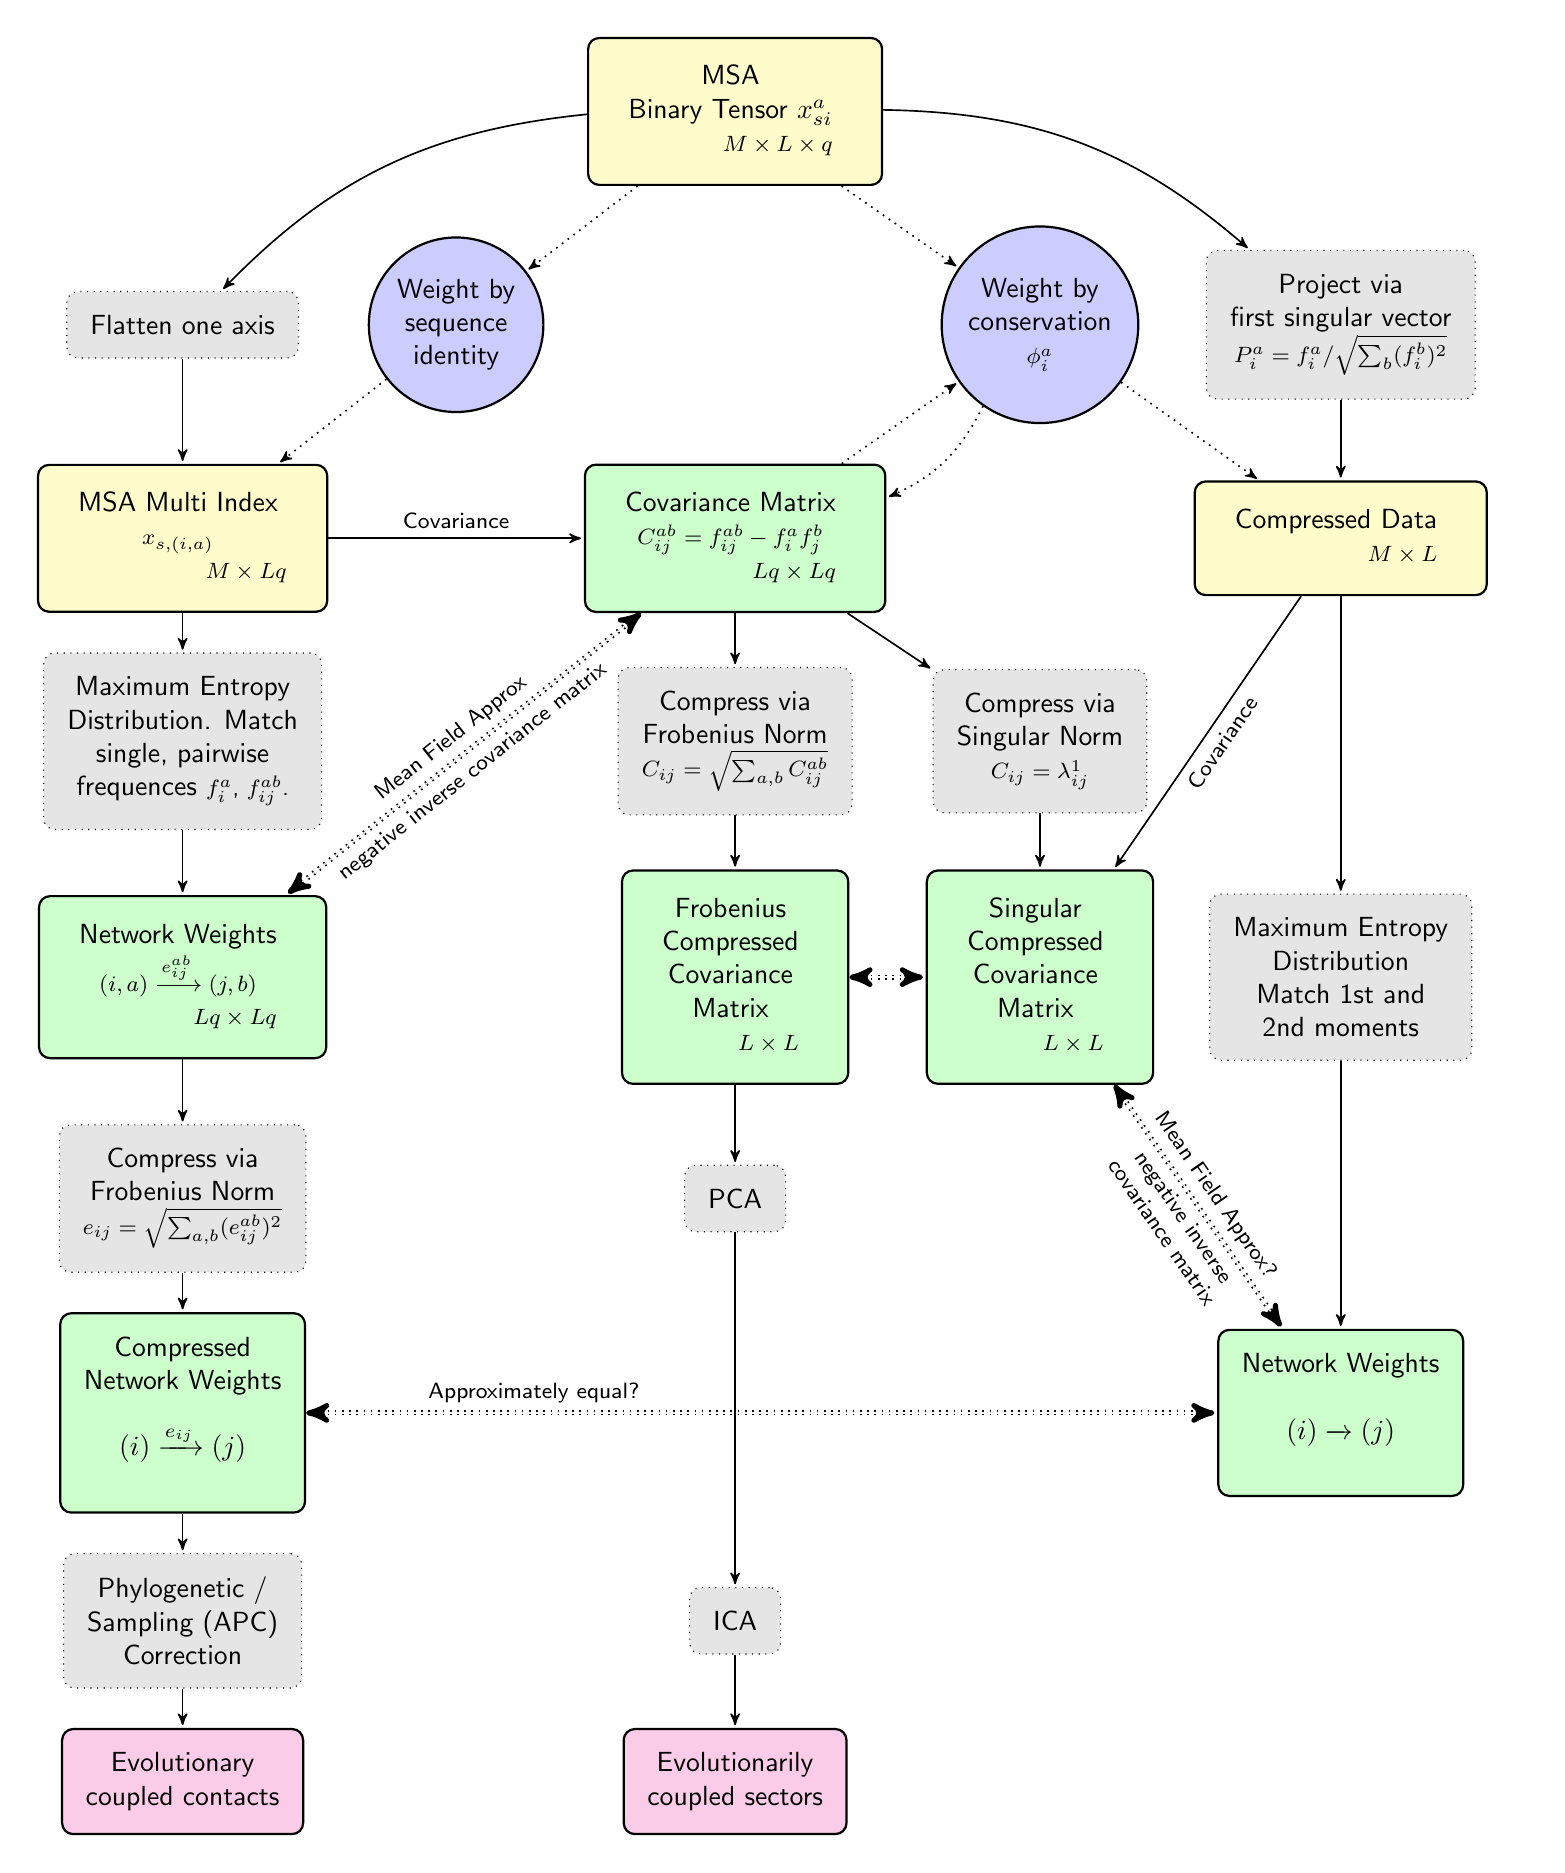
\begin{tikzpicture}[
  font=\sffamily,
  every matrix/.style={ampersand replacement=\&,column sep=.5cm,row sep=.5cm},
  datamat/.style={draw,thick,rounded corners,fill=yellow!20,inner sep=.3cm},
  process/.style={draw,thick,circle,fill=blue!20},
  calcmat/.style={datamat,fill=green!20},
  calcmatfinal/.style={datamat,fill=magenta!20},
  algoprocess/.style={datamat,thin,dotted,fill=gray!20,inner sep=.3cm},
  to/.style={->,>=stealth',shorten >=1pt,semithick,font=\sffamily\footnotesize},
  todots/.style={->,dotted,>=stealth',shorten >=1pt,semithick,font=\sffamily\footnotesize},
  toapprx/.style={<->,double,dotted,>=stealth',shorten >=1pt,semithick,font=\sffamily\footnotesize},
  every node/.style={align=center}]
% Position the nodes using a matrix layout
  \matrix{

    \&
    \&  \node[datamat] (MSA) {
            \begin{tabular}{c}
                MSA \\
                Binary Tensor $x_{si}^a$ \\ 
                \multicolumn{1}{r}{\sffamily\footnotesize $M\times L \times q$}
            \end{tabular}
        }; 
    \&
    \& \\

    \node[algoprocess] (FlattenAxis) {Flatten one axis}; 
    \& \node[process] (weightseqid) {
                Weight by \\ sequence \\ identity
        }; 
    \& 
    \& \node[process] (weightcons) {
            Weight by \\ conservation \\ \sffamily\footnotesize{$\phi_i^a$}
        }; 
    \& \node[algoprocess] (SingularProj)  {
            Project via \\ 
            first singular vector \\ 
            \footnotesize{$P_i^a = {f_i^a}/ {\sqrt{\sum_{b} (f_i^b)^2}}$}
    }; \\

    \node[datamat] (FlattenMSA) {
            \begin{tabular}{c}
            MSA Multi Index \\ 
            \footnotesize{$x_{s, (i,a)}$}\\
            \multicolumn{1}{r}\sffamily\footnotesize{$M\times Lq$}
            \end{tabular}
    };  
    \& 
    \& \node[calcmat] (CovMat) {
            \begin{tabular}{c}
            Covariance Matrix \\ 
            \footnotesize{$C_{ij}^{ab} = f_{ij}^{ab} - f_i^a f_j^b$} \\
            \multicolumn{1}{r}{\sffamily\footnotesize $Lq\times Lq$}
            \end{tabular}
        };
    \&
    \& \node[datamat] (DataProj) {
            \begin{tabular}{c}
            Compressed Data \\
            \multicolumn{1}{r}{\sffamily\footnotesize $M\times L$}
            \end{tabular}
        }; \\


    \node[algoprocess] (MaxEntBig) {
            Maximum Entropy \\
            Distribution. Match \\
            single, pairwise \\
            frequences \footnotesize{$f_i^a$, $f_{ij}^{ab}$}.
        };  
    \& 
    \& \node[algoprocess] (CompressCovFrob) {
            Compress via\\
            Frobenius Norm \\
            \footnotesize{$C_{ij} = \sqrt{\sum_{a,b} C_{ij}^{ab}}$}
        };
    \& \node[algoprocess] (CompressCovSing) {
            Compress via\\
            Singular Norm \\
            \footnotesize{$C_{ij} = \lambda_{ij}^1$}
        };
        \&
    \& \\


    \node[calcmat] (NetworkBig) {
            \begin{tabular}{c}
            Network Weights \\ 
            \footnotesize{$(i,a) \xrightarrow{e_{ij}^{ab}} (j,b)$}  \\
            \multicolumn{1}{r}{\sffamily\footnotesize $Lq\times Lq$}
            \end{tabular}
        };  
    \& 
    \& 
    \node[calcmat] (CompressCovmatFrob) {
            \begin{tabular}{c}
            Frobenius \\ Compressed\\ Covariance \\Matrix\\ 
            \multicolumn{1}{r}{\sffamily\footnotesize $L\times L$}
            \end{tabular}
        };
    \&
    \node[calcmat] (CompressCovmatSing) {
            \begin{tabular}{c}
            Singular \\ Compressed \\ Covariance \\ Matrix \\ 
            \multicolumn{1}{r}{\sffamily\footnotesize $L\times L$}
            \end{tabular}
        };
    \& \node[algoprocess] (MaxEntSmall) {
            Maximum Entropy \\Distribution\\ Match 1st and \\ 2nd moments
        };  
    \\

    \node[algoprocess] (CompressFrob) {
            Compress via\\ Frobenius Norm \\
            \footnotesize{$e_{ij} = {\sqrt{\sum_{a,b} (e_{ij}^{ab})^2}}$}
    };
    \&
    \&
    \node[algoprocess] (PCA) {PCA};
    \& \\

    \node[calcmat] (NetworkBigSmall) {
            Compressed \\ Network Weights \\ \\ $(i) \xrightarrow{e_{ij}} (j)$ \\ 
        };  
    \&  
    \&  
    \&     
    \& \node[calcmat] (NetworkSmall) {
            Network Weights \\ \\ $(i) \xrightarrow{} (j)$ \\ 
        };  
    \\

    \node[algoprocess] (APC) {
            Phylogenetic / \\ Sampling (APC)\\Correction
        };
    \&  
    \&  
    \node[algoprocess] (ICA) {ICA};
    \&  
    \&   \\


    \node[calcmatfinal] (Contacts) {Evolutionary \\coupled contacts};
    \&  
    \&  
    \node[calcmatfinal] (Sectors) {
            Evolutionarily \\ coupled sectors
    }; 
    \&  
    \&   \\
  };

  % Draw the arrows between the nodes and label them.
  \draw[to]     (MSA) to[bend right=20] 
                (FlattenAxis);
  \draw[to]     (FlattenAxis)       --  (FlattenMSA);
  \draw[to]     (MSA) to[bend left=20]             
                (SingularProj);
  \draw[to]     (SingularProj)      --  (DataProj);
  \draw[todots] (MSA)               --  (weightseqid);
  \draw[todots] (MSA)               --  (weightcons);
  \draw[todots] (weightseqid)       --  (FlattenMSA);
  \draw[to]     (FlattenMSA) to 
                    node[midway,above]{Covariance}
                (CovMat);
  \draw[to]     (DataProj) to 
                    node[midway,below,sloped]{Covariance}
                (CompressCovmatSing);
  \draw[todots] (CovMat)            --  (weightcons);
  \draw[todots] (weightcons)        --  (DataProj);
  \draw[to]     (FlattenMSA)        --  (MaxEntBig);
  \draw[to]     (CovMat)            --  (CompressCovFrob);
  \draw[to]     (CovMat)            --  (CompressCovSing);
  \draw[to]     (CompressCovSing)   --  (CompressCovmatSing);
  \draw[todots] (weightcons)    to[bend left=20]  
                (CovMat);
  \draw[to]     (DataProj)          --  (MaxEntSmall);
  \draw[to]     (MaxEntBig)         --  (NetworkBig);
  \draw[to]     (MaxEntSmall)       --  (NetworkSmall);
  \draw[to]     (NetworkBig)        --  (CompressFrob);
  \draw[to]     (CompressCovFrob)   --  (CompressCovmatFrob);
  \draw[to]     (CompressCovmatFrob)--  (PCA);
  \draw[to]     (PCA)               --  (ICA);
  \draw[toapprx](CompressCovmatFrob)--  (CompressCovmatSing);
  \draw[toapprx](CompressCovmatSing) to
                    node[midway,above,sloped] {Mean Field Approx?} 
                    node[midway,below,sloped] {
                            negative inverse \\covariance matrix
                    } 
                (NetworkSmall);
  \draw[to]     (ICA)            --  (Sectors);
  \draw[toapprx](NetworkBigSmall)   to
                    node[near start,above,sloped]{Approximately equal?}
                (NetworkSmall);
  \draw[toapprx](CovMat)        to 
                    node[midway,above,sloped] {Mean Field Approx} 
                    node[midway,below,sloped] {
                            negative inverse covariance matrix
                    } 
                (NetworkBig);
  \draw[to]     (CompressFrob)      -- (NetworkBigSmall);
  \draw[to]     (NetworkBigSmall)   -- (APC);
  \draw[to]     (APC)               -- (Contacts);
\end{tikzpicture}
\caption{Right column shows connection between DCA (leftmost column) and SCA (middle column)}
\end{figure}
\end{document}
